\section{ZTF survey} \label{sec:ztf}
In this section we present the Zwicky Transient Facility survey as well as the the supernova sample that was primarily studied in this PhD the ZTF DR2. The ZTF camera is mounted on the Samuel Oschin 
48-inch (1.2m) telescope in the Mount Palomar Obsrevatory, California, USA. The primary purpose of the survey is the study of nearby astrophysical transients, which makes it 
really good for studying supernovae in the local Universe. \\

\begin{figure}[ht]
    \centering
    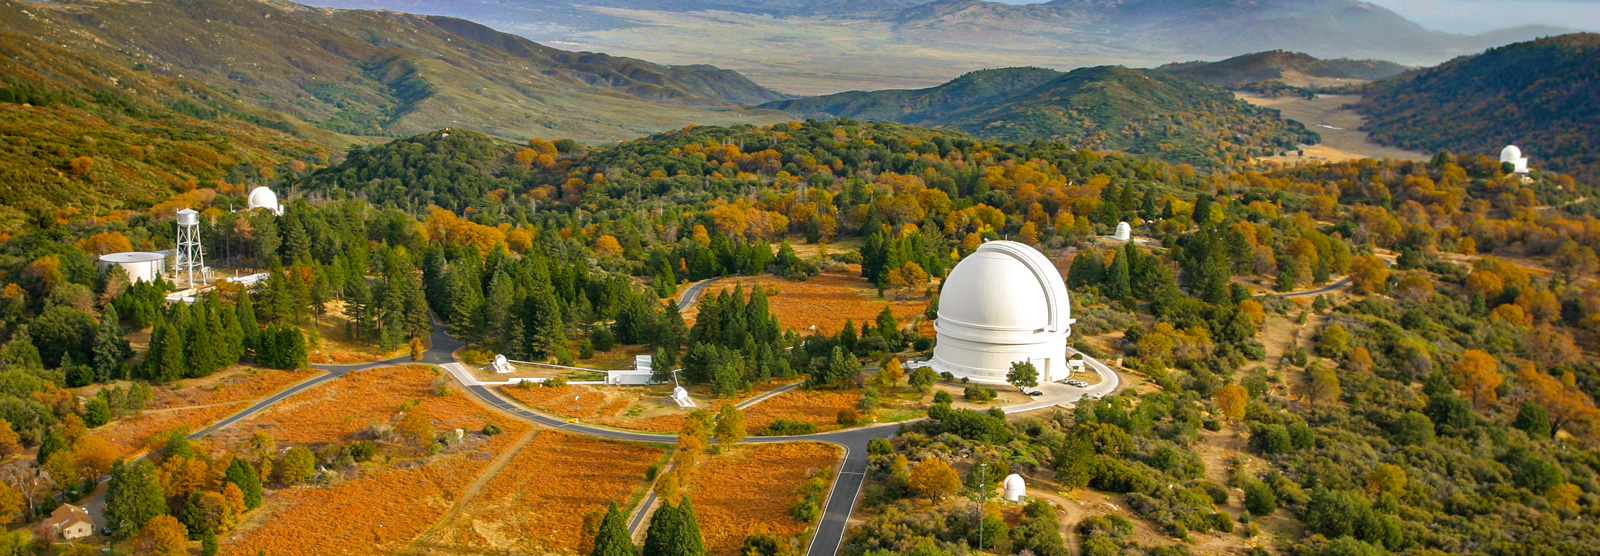
\includegraphics[width=1.0\textwidth]{MainLayout/Second_chapter/figures/palomar-observatory.jpg}
    \caption{Mount Palomar Observatory. Credits: Caltech \url{https://www.ztf.caltech.edu/} }
    \label{fig:palomar}
\end{figure}

\subsection{ZTF photometry}

The ZTF camera is made up of 16 CCDs (model e2v CCD231-C6) each possessing 6144 $\times$ 6160 pixels. The Samuel Oschin telescope contains a 1.2m mirror (called the "primary mirror" M1) that redirects the 
photons to the focal plane of the camera. The mirror is a spherical pyrex-glass mirror coated with aluminium which allows for a large observation field of view. 
The telescope also contains an aspherical lens at the entrance to correct for geometric aberrations. 
It covers a solid angle of $\sim 47 \text{deg}^2$ of the extragalactical northern sky and manages to conduct a full sky coverage twice per night. Each image covers approximately 235 times the area of the full moon. 
The photometry is done using 3 filters $g$, $r$ and $i$ covering the ranges of $\approx 4000 - 5500 \AA$, $\approx 5500 - 7000 \AA$ and $\approx 7000 - 9000 \AA$ respectively. 
It is important to highlight that the transmissions of the filters are sensor-dependent and we display them by averaging over the sensor transmissions. 
The magnitude limits for each band are $m_g \sim 20.8-21.1$mag, $m_r \sim 20.6-20.9$mag, $m_i \sim 19.9-20.2$mag where the variations are laregly due to the phases of the moon. 
The full details on the ZTF photometry are in \cite{Dekany_2020}. \\

\begin{figure}[ht]
    \centering
    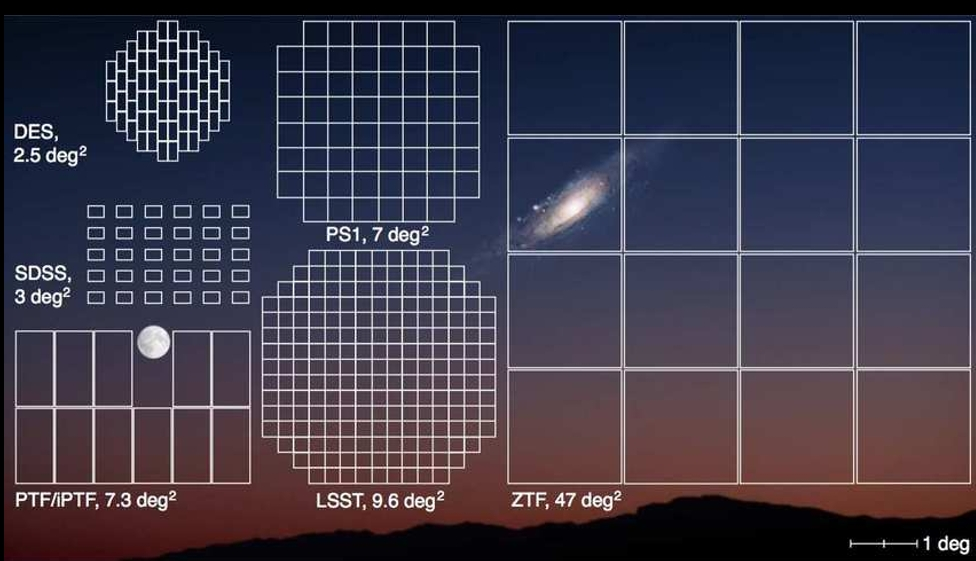
\includegraphics[width=0.8\textwidth]{MainLayout/Second_chapter/figures/ztf-camera-fov.jpg}
    \caption{Comparisons between the fields of view of ZTF, PS1, LSST, PTF, SDSS and DES. In the background we see in comparison the size of the moon and the Andromeda galaxy. Credits: Caltech \url{https://www.ztf.caltech.edu/} }
    \label{fig:ztf_fov}
\end{figure}

\begin{figure}[ht]
    \centering
    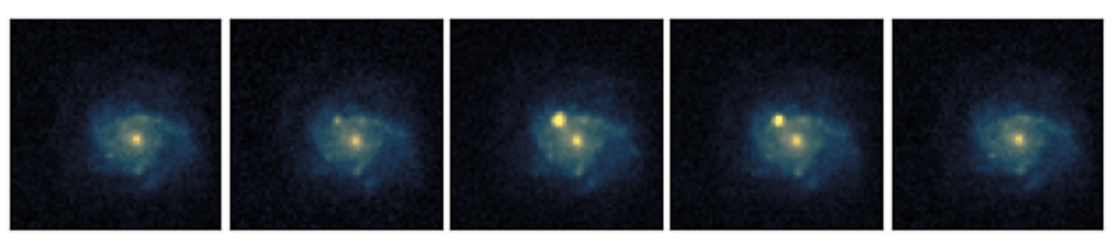
\includegraphics[width=1.0\textwidth]{MainLayout/Second_chapter/figures/ztf_sn_picture.png}
    \caption{Type Ia supernova detected by ZTF. Photos taken accross 2 months (from left to right 20th of Jan 2020, 25th of Jan 2020, 7th of Feb 2020, 20th of Feb 2020, 20th of March 2020). Credits: Mikaël Rigault.}
    \label{fig:ztf_sn_picture}
\end{figure}

\begin{figure}[ht]
    \centering
    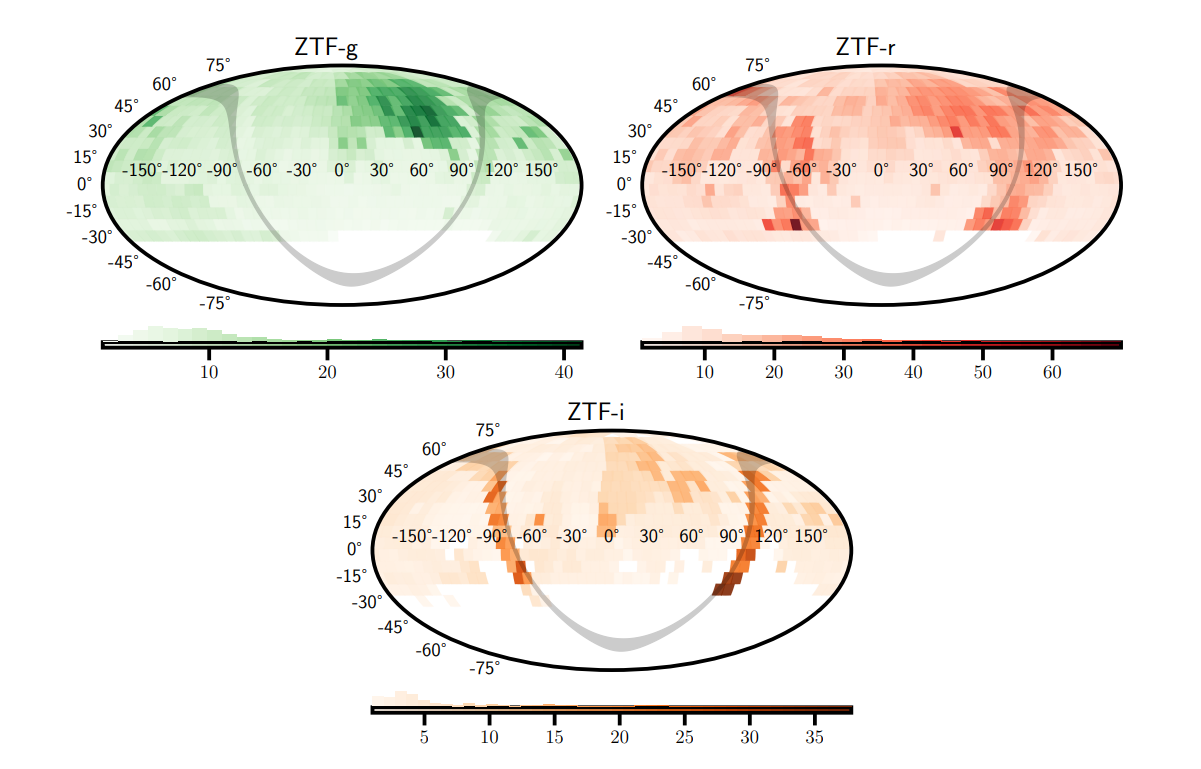
\includegraphics[width=0.8\textwidth]{MainLayout/Second_chapter/figures/ztf_cadence.png}
    \caption{ZTF cadence on the sky. Average number of visits per month for each field of ZTF in each band $g$, $r$ and $i$. Taken from \cite{Carres_2023}}
    \label{fig:ztf_cadence}
\end{figure}

\begin{figure}[ht]
    \centering
    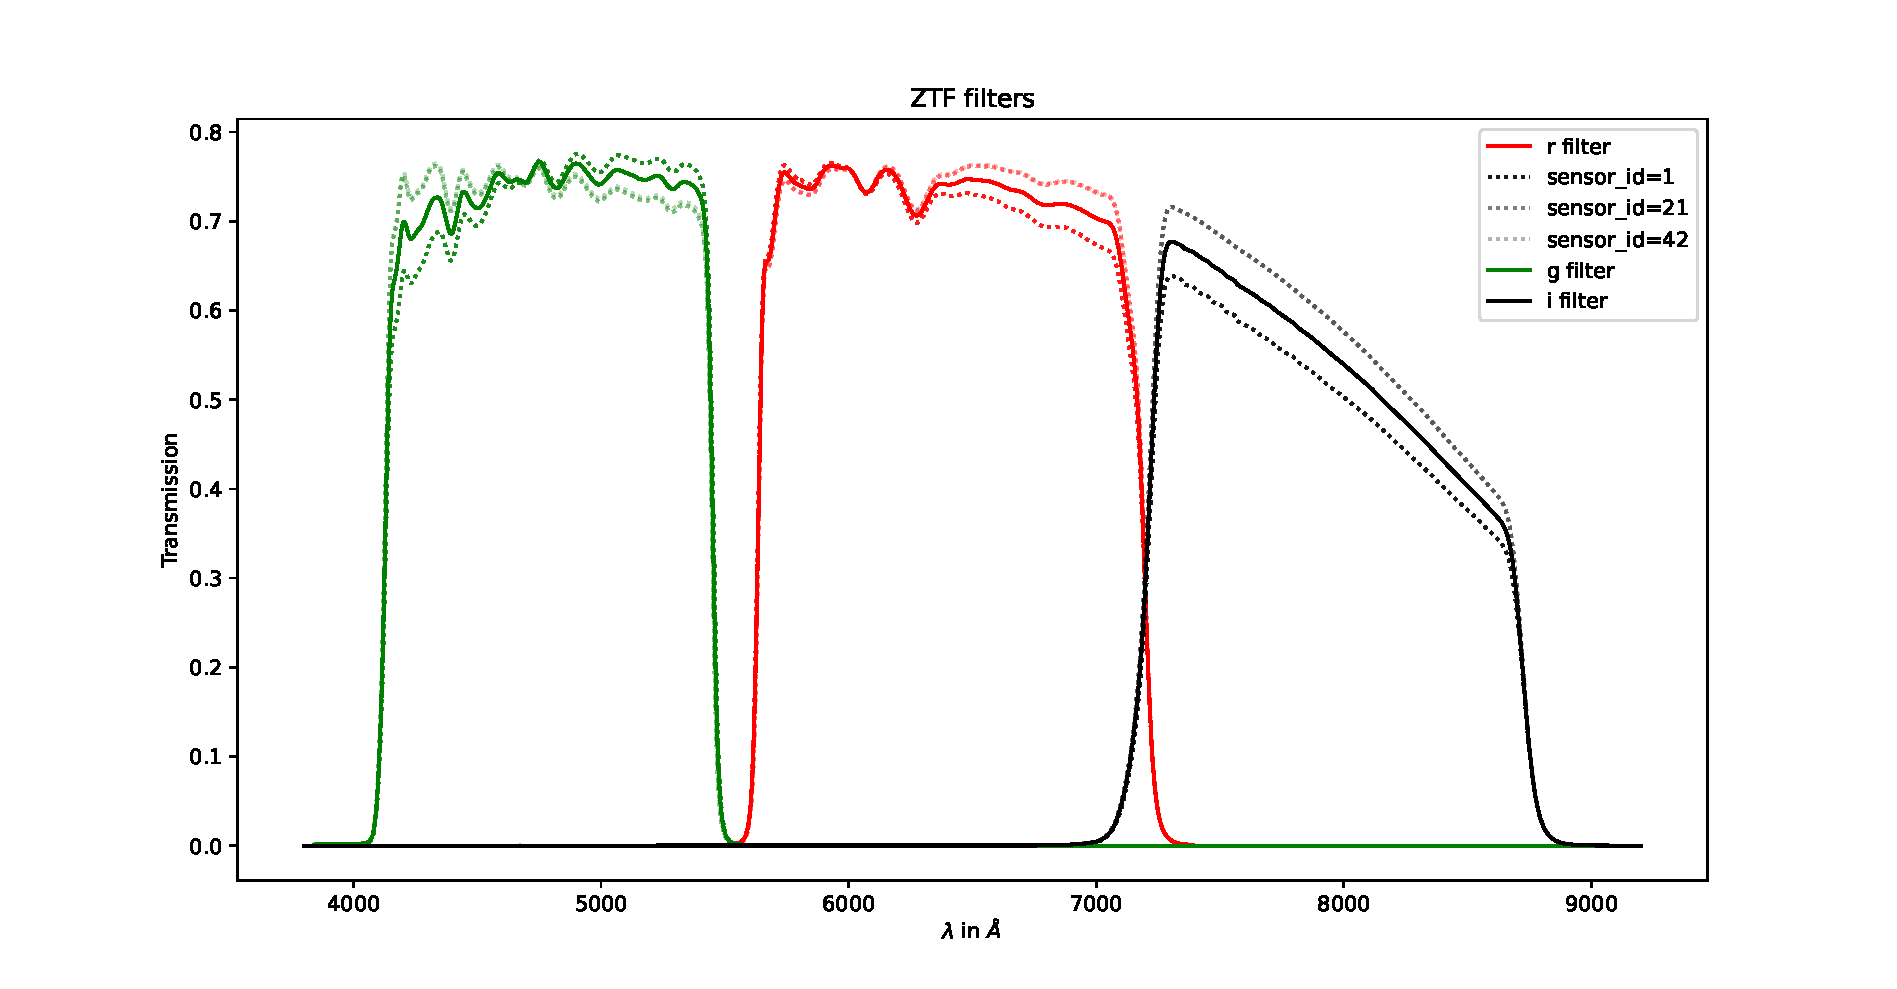
\includegraphics[width=1.0\textwidth]{MainLayout/Second_chapter/figures/ztf_filters.pdf}
    \caption{ZTF filters. Dotted lines represent transmissions for different sensors. Solid lines represent the average transmissions over all sensors.}
    \label{fig:ztf_cadence}
\end{figure}

\subsection{Spectroscopic follow up}

ZTF is accompagnied by a spectrograph named the Spectral Energy Distribution Machine (SEDM) located in the same observatory on the P60 telescope. The purpose of the object to 
conduct a follow up on the photometry in order to properly classify the transients obsereved. It's limit magnitude is 20.5mag. This follow up played an important role in acquiring the 
60\% spectra for the ZTF Bright Transient Survey (BTS) for which the magnitude limit was 18.5mag, a limited fraction of the ZTF total survey. \\


\subsection{ZTF DR2}

We present in this subsection the type Ia supernova data release of ZTF named DR2. This encompasses data taken from March 2018 and December 2020. The sample contains 3628 
spectroscopically identified supernovae up to a redshift of $z \approx 0.2$. Figure \ref{fig:ztf_lcs} shows examples of the sampling of the supernova obsereved by ZTF in DR2. We must note that not all supernova data is 
"good" enough to be used for a cosmological analysis. For such an analysis, quality cuts on sampling around the maximum emission of light, the color and the stretch must be applied. 
The details on the cosmology quality cuts can be found in \cite{Rigault_2020} and we remind them later in Chapter 4. After the cuts, 
the sample maintains 2667 supernovae that pass. A subset of the sample named the "volume-limited" sample contains all supernovae up to a redshift of $z=0.06$ represents a complete 
sample of supernovae i.e. the sample is not influenced by any selection effects due to the magnitude limits of the telescope. This subset contains 994 supernovae. \\

\begin{figure}[ht]
    \centering
    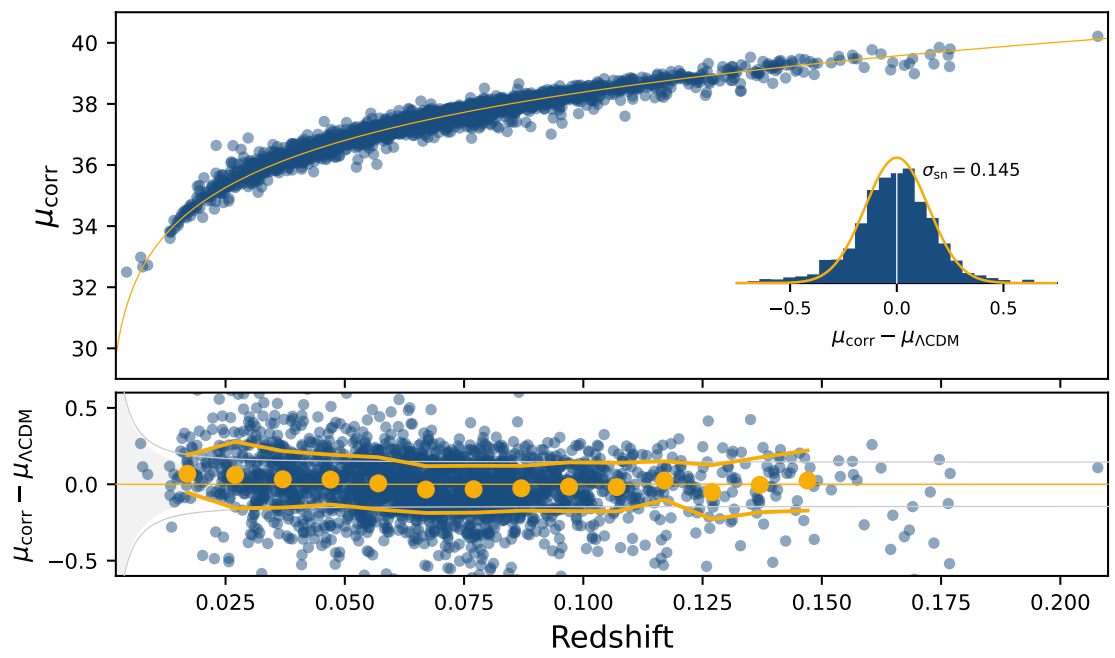
\includegraphics[width=0.8\textwidth]{MainLayout/Second_chapter/figures/ztf_dr2_hubble.png}
    \caption{Hubble diagram created with standardized ZTF DR2 type Ia supernovae compared to fiducial $\Lambda$CDM cosmology anchore on Planck results. Taken from \cite{Rigault_2020}.}
    \label{fig:ztf_dr2_hubble}
\end{figure}

\begin{figure}[ht]
    \centering
    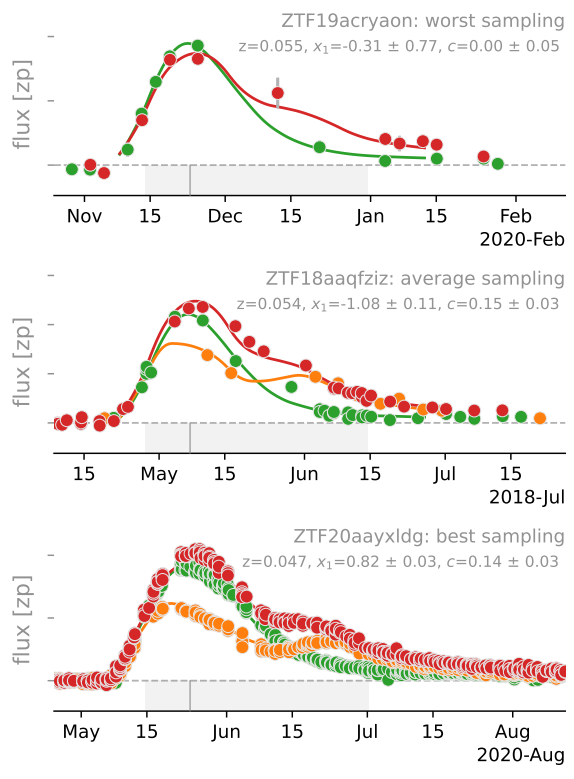
\includegraphics[width=0.5\textwidth]{MainLayout/Second_chapter/figures/ztf_sn_dr2.png}
    \caption{Three supernova Ia lightcurves examples highlighting the worst (top), average (middle) and best (bottom) sampling in DR2. The colors indicate the band they were measured in and the solid lines are the best SALT2 fits. Taken from \cite{Rigault_2020}}
    \label{fig:ztf_lcs}
\end{figure}



\section{DESI survey}

In this section, we briefly present the Dark Energy Spectroscopic Instrument (DESI). This novel, fully robotic instrument, has allowed us to observe the Universe in great detail and 
proven to being capable of adding insight to our understanding of the accelerated Universe (\cite{DESI_DR2_2025}). 
In april 2026, DESI completed its main observation sequence and covered $14000\text{deg}^2$ with over 60 million objects (with 47 million galaxies and quasars) observed within 5 years. \\

\subsection{Spectroscopic instrument}

DESI is a fourth-generation spectroscopic survey. It is a robotic fibre-fed spectroscopic instrument. 
It is installed on the 4-meter Mayall telescope at Kitt Peak National Observatory in Arizona, USA. 
It contains 5000 fibres, each able to observe a separate spectrum, allowing the instrument to gather 5000 spectra at a time, covering for one exposure around $3 \text{deg}^2$
part of the sky. This is a great improvement over its predecessor SDSS (\cite{Dawson_2016}) which had 1000 fibres positioned manually, therefore taking a lot more time than DESI. 
The DESI spectrograph covers a range of $3600-9800 \AA$ where the light is divided into three wavelength channels: Blue ($b$), Red ($r$) and Near Infrared ($Z$). Finally, the light 
is captured by CCDs installed in a vacuum cryostat. Two different CCD models are used: STA4150 (4096 $\times$ 4096 pixels) and CCDs produced by LBL specifically for DESI 
(4114 $\times$ 4128 pixels). More details on the instrument can be found here \cite{DESI_Instrument_2016}.\\

\subsection{Tracers}

DESI catalogues its observations under multiple classes each presenting a of matter tracer in the observable Universe (\cite{DESI_Design_2016}).

\noindent \textbf{\underline{BGS}} \\

The first catalogue is the Bright Galaxy Survey (BGS). It is a flux limited galaxy catalogue that is divided into two parts based in the magntidue of the obsereved galaxy. BGS 
Bright contains galaxies with magnitudes in the $r$ band $<19.5$ and BGS faint with magnitudes $19.5 - 20.175$, these are present at a redshift range of $z<0.6$. To identify if the obsereved object is a galaxy or a star it is 
cross references with the Gaia catalogue. If it is not present then it is a galaxy. There are over 10 million galaxies in the BGS catalogue. These also present the galaxies closest to us. \\

\noindent \textbf{\underline{LRG}} \\

The second catalogue is the Luminous Red Galaxies (LRG) which contains old elliptical galaxies, identified due the $4000\AA$ break line in their spectra, in which 
the star formation rate has stopped. The LRG present galaxies in the redshift range $0.4<z<1.0$.

\noindent \textbf{\underline{ELG}} \\

The third catalogue is the Emission Line Galaxies (ELG) which contains younger spiral galaxies with star formation. It is divided into two subcategories: ELG VLOP with galaxies 
at redshifts $0.6<z<1.1$ and ELG LOP with galaxies at $1.1<z<1.6$. \\ 

\noindent \textbf{\underline{QSO}} \\

The fourth catalogue is the Quasar-Stellar Objects (QSO). The catalogue contains quasars, active galactic nuclei which are powered by the accretion of super massive black holes. 
The quasars measured at a redshift of $0.9<z<2.1$ are used as direct matter tracers, while quasars at $2.1<z<4.0$ will be used for their Lyman-$\alpha$ forest. This 
represents the furthest objects obsereved by DESI. \\

DESI at the time of writing this thesis has entered an extension phase of observation until 2028 where the sky coverage will go up to $17000\text{deg}^2$. \\

\subsection{ZTF and DESI Synergies}

ZTF and DESI present two of the current generation surveys that will tackle known tensions in the cosmological model. In addition to that, ZTF's sky coverage is in fact encompassed 
by DESI's coverage and the BGS sample is actually present at the same redshift range as ZTF. This creates synergies between the surveys that could explored.\\ 
Firstly, DESI's spectroscopic instrument has more accurate measurements of redshifts than the SEDM, therefore redshifts provided by DESI to ZTF can improve 
the mapping of the expanding history of the Universe using supernovae. They will also provide more accurate measurements of growth rate of structures 
using ZTF since it heavily relies on comparing the observed redshift to the cosmological redshift due to the expansion (see Section \ref{sec:vp_methods}). \\ 
Secondly, the BGS Bright sample contains galaxies in the same redshift range as the ZTF DR2. This highly favours conducting cross-survey analyses, which is the main 
goal of this PhD regarding the measurement of the growth rate of structures $f\sigma_8$. The DESI growth rate of structure measurements at low redshift is limited by the cosmic 
variance (the statistical uncertainty that arises due to only having access to one realization of the Universe) and galaxy bias. Supernova measurements can directly probe 
the underlying velocity field (see Section \ref{sec:vp_methods}) independently of any galaxy bias. Therefore a combination of both DESI and ZTF is projected to yield more 
precise measurements of $f\sigma_8$ at a low redshift. This is particularly important since the measurement of the growth rate of structures is a direct test of GR and is most 
sensitive at low redshift. \\
